\documentclass[tikz,border=10pt]{standalone}
\usepackage{amsmath}
\usetikzlibrary{arrows.meta, positioning, calc, fit, decorations.pathreplacing}

\definecolor{c1}{HTML}{000000}  % black       - structure, axes
\definecolor{c2}{HTML}{233D4D}  % deep slate  - the windows we impose, matrices
\definecolor{c3}{HTML}{FE7F2D}  % orange      - the measurements themselves
\definecolor{c4}{HTML}{EAECF0}  % cool grey   - panel fills
\definecolor{axiscolor}{HTML}{333333}
\definecolor{labelcolor}{HTML}{5F6B75}

\begin{document}
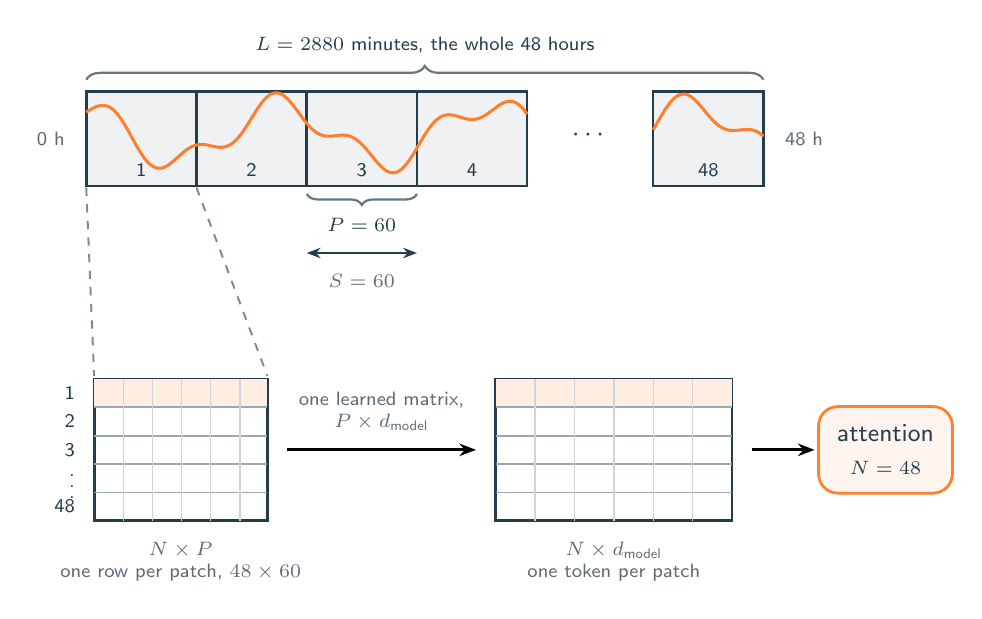
\begin{tikzpicture}[
    every node/.style={font=\sffamily},
    patch/.style={
        rectangle, draw=c2, fill=c2!7, line width=0.9pt,
    },
    arr/.style={-{Stealth[length=6pt]}, line width=1.1pt, color=c1},
    dbl/.style={{Stealth[length=5pt]}-{Stealth[length=5pt]}, line width=0.9pt, color=c2},
    lab/.style={font=\sffamily\scriptsize, text=labelcolor},
    tag/.style={font=\sffamily\scriptsize, text=c2},
    guide/.style={c2!60, line width=0.7pt, dashed},
]

% ============================================================ the whole stretch
\draw[decorate, decoration={brace, amplitude=5pt}, c2!70, line width=0.8pt]
    (0.80, 7.50) -- (9.40, 7.50)
    node[midway, above=6pt, font=\sffamily\scriptsize, text=c2]
    {$L = 2880$ minutes, the whole 48 hours};

% the four leading patches, then the last one
\foreach \a/\b/\n in {0.80/2.20/1, 2.20/3.60/2, 3.60/5.00/3, 5.00/6.40/4}{
    \draw[patch] (\a, 6.15) rectangle (\b, 7.35);
    \node[tag] at ({(\a+\b)/2}, 6.35) {\n};
}
\draw[patch] (8.00, 6.15) rectangle (9.40, 7.35);
\node[tag] at (8.70, 6.35) {48};
\node[text=c2] at (7.20, 6.80) {$\cdots$};

% the signal itself, cut by nothing: the windows are ours, not its
\draw[c3, line width=1.1pt]
    plot[domain=0.80:6.40, samples=180, smooth]
    (\x, {6.82 + 0.36*sin(\x r * 2.4) + 0.16*sin(\x r * 6.1 + 55)});
\draw[c3, line width=1.1pt]
    plot[domain=8.00:9.40, samples=60, smooth]
    (\x, {6.82 + 0.36*sin(\x r * 2.4) + 0.16*sin(\x r * 6.1 + 55)});

\node[lab, anchor=east] at (0.65, 6.75) {0 h};
\node[lab, anchor=west] at (9.55, 6.75) {48 h};

% P, the length of one patch
\draw[decorate, decoration={brace, amplitude=4pt, mirror}, c2!70, line width=0.8pt]
    (3.60, 6.05) -- (5.00, 6.05)
    node[midway, below=5pt, font=\sffamily\scriptsize, text=c2] {$P = 60$};

% S, the distance from one start to the next
\draw[dbl] (3.60, 5.30) -- (5.00, 5.30);
\node[lab, anchor=north] at (4.30, 5.16) {$S = 60$};

% ============================================================ patch 1 becomes row 1
\draw[guide] (0.80, 6.13) -- (0.90, 3.74);
\draw[guide] (2.20, 6.13) -- (3.10, 3.74);

% ============================================================ the matrix of patches
\draw[c2, line width=1.0pt] (0.90, 1.90) rectangle (3.10, 3.70);
\fill[c3!14] (0.90, 3.34) rectangle (3.10, 3.70);
\foreach \y in {3.34, 2.98, 2.62, 2.26}{
    \draw[c2!45, line width=0.6pt] (0.90, \y) -- (3.10, \y);
}
\foreach \x in {1.27, 1.64, 2.01, 2.38, 2.75}{
    \draw[c2!22, line width=0.5pt] (\x, 1.90) -- (\x, 3.70);
}
\node[tag, anchor=east] at (0.78, 3.52) {1};
\node[tag, anchor=east] at (0.78, 3.16) {2};
\node[tag, anchor=east] at (0.78, 2.80) {3};
\node[tag, anchor=east] at (0.78, 2.44) {$\vdots$};
\node[tag, anchor=east] at (0.78, 2.08) {48};
\node[lab, anchor=north, align=center] at (2.00, 1.75)
    {$N \times P$\\ one row per patch, $48 \times 60$};

% ============================================================ the projection
\draw[arr] (3.35, 2.80) -- (5.75, 2.80);
\node[lab, anchor=south, align=center] at (4.55, 2.92)
    {one learned matrix,\\ $P \times d_{\text{model}}$};

% ============================================================ the token sequence
\draw[c2, line width=1.0pt] (6.00, 1.90) rectangle (9.00, 3.70);
\fill[c3!14] (6.00, 3.34) rectangle (9.00, 3.70);
\foreach \y in {3.34, 2.98, 2.62, 2.26}{
    \draw[c2!45, line width=0.6pt] (6.00, \y) -- (9.00, \y);
}
\foreach \x in {6.50, 7.00, 7.50, 8.00, 8.50}{
    \draw[c2!22, line width=0.5pt] (\x, 1.90) -- (\x, 3.70);
}
\node[lab, anchor=north, align=center] at (7.50, 1.75)
    {$N \times d_{\text{model}}$\\ one token per patch};

% ============================================================ attention
\draw[arr] (9.25, 2.80) -- (10.05, 2.80);
\node[
    rectangle, rounded corners=7pt, minimum width=1.7cm, minimum height=1.1cm,
    draw=c3, fill=c3!8, text=c2, line width=1.0pt, align=center,
    font=\sffamily\small
] at (10.95, 2.80) {attention\\[1pt] \scriptsize $N = 48$};

\end{tikzpicture}
\end{document}
